\section{ESP32}

Embedded System Processors (ESP) are versatile microcontroller units (MCUs) widely used in Internet of Things (IoT) and embedded applications. Developed by Espressif Systems, these modules combine powerful processing with Wi-Fi and Bluetooth connectivity, making them ideal for smart home devices, wearables, and industrial automation.

\begin{figure}[h!]
	\centering
	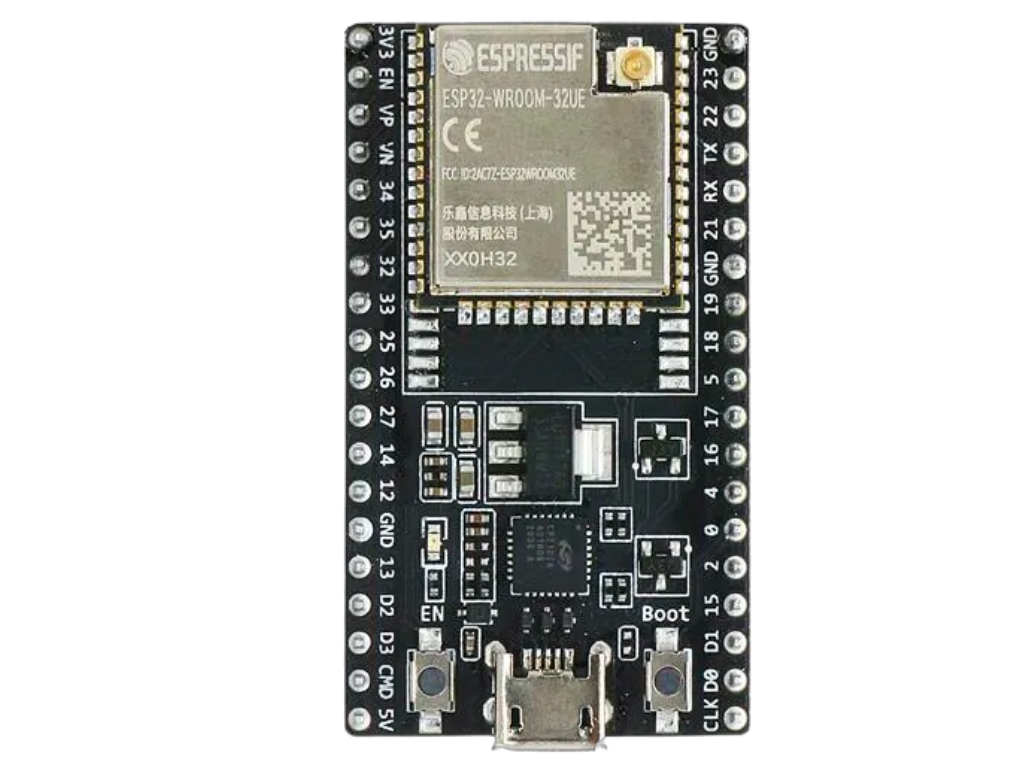
\includegraphics[width=0.4\linewidth]{assets/ch2/esp32}
	\caption{ESP32-WROOM Development board}
	\label{fig:esp32}
\end{figure}

\subsection{ESP Series Overview}

The ESP series includes different models tailored to specific application needs for performance, power efficiency, and connectivity. Key types include:

\begin{itemize}
	\item \textbf{ESP8266 Series:} A cost-effective option with a 32-bit LX6 single-core processor (up to 160 MHz), supporting 2.4 GHz Wi-Fi and peripheral interfaces like UART, I2C, and PWM. Its low power consumption suits battery-powered applications.
	
	\item \textbf{ESP32 Series:} Offers more power and connectivity. The ESP32-S2 has a single-core LX7 processor, while the ESP32-S3 features a dual-core LX7 processor (up to 240 MHz), with 2.4 GHz Wi-Fi and Bluetooth 5.0. It includes security features like secure boot and flash encryption.
	
	\item \textbf{ESP32-S2 Series:} A low-power option with a single-core LX7 processor (up to 240 MHz) and Wi-Fi support. It includes USB OTG and advanced security features, making it suitable for secure IoT applications.
	
	\item \textbf{ESP32-S3 Series:} Designed for AI and neural network applications, it features a dual-core LX7 processor (up to 240 MHz), with Wi-Fi and Bluetooth 5 (LE). It has added vector instructions for AI tasks and comprehensive security options.
\end{itemize}

\subsection{Key Features of ESP Modules}

ESP modules provide a range of features for various applications:

\begin{itemize}
	\item \textbf{Processing Power:} 32-bit processors with single or dual cores, running between 160 and 240 MHz.
	
	\item \textbf{Wireless Connectivity:} All modules support 2.4 GHz Wi-Fi; some also include Bluetooth 5.0 (LE).
	
	\item \textbf{Memory and Storage:} Includes SRAM and ROM, with options to add external flash and PSRAM. The ESP32-S3, for instance, has up to 512 KB SRAM and supports various SPI interfaces.
	
	\item \textbf{Peripherals and Interfaces:} Offers GPIO, SPI, I2C, I2S, UART, PWM, ADC, DAC, and USB OTG (on select models), supporting a wide variety of sensors and devices.
	
	\item \textbf{Power Efficiency:} Low-power modes and fine-grained control make ESP modules suitable for battery-powered devices, with the ESP32-S2 optimized for ultra-low-power applications.
\end{itemize}

With their range of types, processors, and features, ESP modules offer a flexible solution for IoT and embedded systems, meeting the needs of modern, connected applications.
